\documentclass{beamer}
\usepackage[utf8]{inputenc}

\usetheme{Madrid}
\usecolortheme{default}
\usepackage{extarrows}
\usepackage{amsmath}
\usepackage{extarrows}
\usepackage{amssymb,amsfonts,amsthm}
\usepackage{txfonts}
\usepackage{tkz-euclide}
\usepackage{listings}
\usepackage{adjustbox}
\usepackage{array}
\usepackage{tabularx}
\usepackage{gvv}
\usepackage{lmodern}
\usepackage{circuitikz}
\usepackage{tikz}
\usepackage{graphicx}
\usepackage{amsmath} 

\setbeamertemplate{page number in head/foot}[totalframenumber]

\usepackage{tcolorbox}
\tcbuselibrary{minted,breakable,xparse,skins}

\definecolor{bg}{gray}{0.95}
\DeclareTCBListing{mintedbox}{O{}m!O{}}{%
  breakable=true,
  listing engine=minted,
  listing only,
  minted language=#2,
  minted style=default,
  minted options={%
    linenos,
    gobble=0,
    breaklines=true,
    breakafter=,,
    fontsize=\small,
    numbersep=8pt,
    #1},
  boxsep=0pt,
  left skip=0pt,
  right skip=0pt,
  left=25pt,
  right=0pt,
  top=3pt,
  bottom=3pt,
  arc=5pt,
  leftrule=0pt,
  rightrule=0pt,
  bottomrule=2pt,
  toprule=2pt,
  colback=bg,
  colframe=orange!70,
  enhanced,
  overlay={%
    \begin{tcbclipinterior}
    \fill[orange!20!white] (frame.south west) rectangle ([xshift=20pt]frame.north west);
    \end{tcbclipinterior}},
  #3,
}
\lstset{
    language=C,
    basicstyle=\ttfamily\small,
    keywordstyle=\color{blue},
    stringstyle=\color{orange},
    commentstyle=\color{green!60!black},
    numbers=left,
    numberstyle=\tiny\color{gray},
    breaklines=true,
    showstringspaces=false,
}
\title %optional
{10.7.97}
\author 
{EE25BTECH11049-Sai Krishna Bakki}

\begin{document}

\frame{\titlepage}
\begin{frame}{Question}
Let $\vec{P}\brak{a \sec \theta, b \tan \theta}$ and $\vec{Q}\brak{a \sec \phi, b \tan \phi}$, where $\theta + \phi = \pi/2$, be two points on the hyperbola $\frac{x^2}{a^2} - \frac{y^2}{b^2} = 1$. If $(h, k)$ is the point of intersection of the normals at $\vec{P}$ and $\vec{Q}$, then $k$ is equal to?
\end{frame}
\begin{frame}{Theoretical Solution}
    The equation of the hyperbola is $\frac{x^2}{a^2} - \frac{y^2}{b^2} = 1$. Following the general form for a conic $g(\vec{x}) = \vec{x}^T \vec{V} \vec{x} + 2\vec{u}^T \vec{x} + f = 0$, we can identify the corresponding matrices and vectors for our hyperbola:
\begin{align}
     \vec{V} = \myvec{b^2 & 0 \\ 0 & -a^2}, 
     \vec{u} = \myvec{0 \\ 0}, 
     f = -a^2b^2
\end{align}
The equation of the normal to the conic at a point of contact $\vec{q}$ is given by:
\begin{align}
 \brak{\vec{V}\vec{q} + \vec{u}}^T \vec{R} \brak{\vec{x} - \vec{q}} = 0 
 \end{align}
where $\vec{R}$ is the 90-degree rotation matrix, $\vec{R} = \myvec{0 & -1 \\ 1 & 0}$.\\
The coordinates are $\vec{P} = \myvec{ a \sec \theta \\ b \tan \theta }$.
The equation of the normal at $\vec{P}$ is:
\begin{align}
   \brak{\vec{V}\vec{P} + \vec{u}}^T \vec{R} \brak{\vec{x} - \vec{P}} = 0 
\end{align}
\end{frame}
\begin{frame}{Theoretical Solution}
\begin{align}
    \myvec{ ab^2 \sec \theta & -a^2b \tan \theta } \myvec{ 0 & -1 \\ 1 & 0 } \myvec{ x - a \sec \theta \\ y - b \tan \theta } &= 0 \\
    \myvec{ -a^2b \tan \theta & -ab^2 \sec \theta } \myvec{ x - a \sec \theta \\ y - b \tan \theta } &= 0\\
    \myvec{a\tan\theta&b\sec\theta}\vec{x}&=(a^2 + b^2) \tan \theta \sec \theta
\end{align}
The coordinates are $\vec{Q} = \myvec{ a \sec \phi \\ b \tan \theta }$.
The equation of the normal at $\vec{Q}$ is:
\begin{align}
    \myvec{ -a^2b \tan \phi & -ab^2 \sec \phi } \myvec{ x - a \sec \phi \\ y - b \tan \phi } &= 0\\
    \myvec{a\tan\phi&b\sec\phi}\vec{x}&=(a^2 + b^2) \tan \phi \sec \phi
\end{align}
\end{frame}
\begin{frame}{Theoretical Solution}
We are given the condition $\theta + \phi = \pi/2$. We can use this to simplify the second equation.
The intersection point $(h, k)$ must satisfy the normal equations for both P and Q.
\begin{align}
    \myvec{a\tan\theta&b\sec\theta}\myvec{h\\k}&=(a^2 + b^2) \tan \theta \sec \theta\\
    \myvec{a\cot\theta&b\csc\theta}\myvec{h\\k}&=(a^2 + b^2) \cot \theta \csc \theta
    \end{align}
We can solve this linear system for the variables $h$ and $k$ by setting up an augmented matrix.
\begin{align}
\augvec{2}{1}{
a\tan\theta & b\sec\theta & (a^2+b^2)\tan\theta\sec\theta \\
a\cot\theta & b\csc\theta & (a^2+b^2)\cot\theta\csc\theta}
\end{align}
Simplifying to $\sin\theta $ and $\cos\theta$:
\begin{align}
 \augvec{2}{1}{
a\sin\theta\cos\theta & b\cos\theta & (a^2+b^2)\sin\theta \\
a\sin\theta\cos\theta & b\sin\theta & (a^2+b^2)\cos\theta
}
\end{align}
\end{frame}
\begin{frame}{Theoretical Solution}
\begin{align}
\xrightarrow{R_2\rightarrow R_2-R_1}
 \augvec{2}{1}{
a\sin\theta\cos\theta & b\cos\theta & (a^2+b^2)\sin\theta \\
0 & b(\sin\theta - \cos\theta) & (a^2+b^2)(\cos\theta - \sin\theta)
}
\end{align}
We get the value of k:  
\begin{align}
    k=\frac{(a^2+b^2)(\cos\theta - \sin\theta)}{b(\sin\theta - \cos\theta)}
\end{align}
Assuming $\theta \neq \pi/4$,
\begin{align}
 k  &= -\frac{a^2 + b^2}{b}
\end{align}
\end{frame}
\begin{frame}[fragile]
\frametitle{C Code}
\begin{lstlisting}
#include <math.h>
// Define a structure to return the (x, y) coordinates
struct Point {
    double x;
    double y;
};
// This function will be exported to the shared library
// It takes hyperbola parameters a, b, and the angle theta
struct Point find_intersection(double a, double b, double theta) {
    // Given condition from the problem
    double phi = M_PI / 2.0 - theta;

    // Coefficients for the equation of the normal at P(theta)
    // from a*tan(theta)*h + b*sec(theta)*k = (a^2+b^2)*tan(theta)*sec(theta)
    double A1 = a * tan(theta);
    double B1 = b / cos(theta);
    double C1 = (a * a + b * b) * tan(theta) / cos(theta);
\end{lstlisting}
\end{frame}
\begin{frame}[fragile]
\frametitle{C Code}
\begin{lstlisting}
    // Coefficients for the equation of the normal at Q(phi)
    // from a*tan(phi)*h + b*sec(phi)*k = (a^2+b^2)*tan(phi)*sec(phi)
    double A2 = a * tan(phi);
    double B2 = b / cos(phi);
    double C2 = (a * a + b * b) * tan(phi) / cos(phi);

    // Solve the 2x2 system of linear equations for h (intersection.x) and k (intersection.y)
    // A1*h + B1*k = C1
    // A2*h + B2*k = C2
    // Using Cramer's rule:
    double determinant = A1 * B2 - A2 * B1;
 \end{lstlisting}
\end{frame}
\begin{frame}[fragile]
\frametitle{C Code}
\begin{lstlisting}   
    struct Point intersection;

    if (determinant != 0) {
        intersection.x = (C1 * B2 - C2 * B1) / determinant;
        intersection.y = (A1 * C2 - A2 * C1) / determinant;
    } else {
        // This case (parallel normals) shouldn't occur for a hyperbola
        intersection.x = NAN; // Not a Number
        intersection.y = NAN;
    }

    return intersection;
}
\end{lstlisting}
\end{frame}
\begin{frame}[fragile]
\frametitle{Python Code Through Shared Output}
\begin{lstlisting}
import ctypes
import numpy as np
import matplotlib.pyplot as plt

# --- 1. SETUP CTYPES INTERFACE ---

# Define a Python class that mirrors the C 'struct Point'.
# This tells Python how to interpret the data returned by the C function.
class Point(ctypes.Structure):
    _fields_ = [("x", ctypes.c_double),
                ("y", ctypes.c_double)]

# Load the compiled C shared library.
# The name must match the file created in the compilation step.
# On Windows, this would be 'intersection.dll'.
# On macOS, it would be 'intersection.dylib'.
try:
    c_lib = ctypes.CDLL('./hyp.so')
    \end{lstlisting}
\end{frame}
\begin{frame}[fragile]
\frametitle{Python Code Through Shared Output}
\begin{lstlisting}
except OSError:
    print("Could not load the C library.")
    exit()
# Define the function signature from the C library for type safety.
# Set the return type of the C function to be our Point structure.
c_lib.find_intersection.restype = Point
# Set the argument types for the C function (three doubles).
c_lib.find_intersection.argtypes = [ctypes.c_double, ctypes.c_double, ctypes.c_double]

# --- 2. PYTHON LOGIC AND VISUALIZATION ---

# Parameters (chosen to match the plot in Figure_1.png)
a = 5.0
b = 3.0
theta = 0.52
\end{lstlisting}
\end{frame}
\begin{frame}[fragile]
\frametitle{Python Code Through Shared Output}
\begin{lstlisting}
# --- Call the C function to perform the calculation ---
# The heavy lifting is now done by the compiled C code.
intersection_result = c_lib.find_intersection(a, b, theta)
h = intersection_result.x
k = intersection_result.y

# --- Verification ---
# Compare the result from C with the theoretical value from main.tex
k_theoretical = -(a**2 + b**2) / b
print("--- Intersection of Normals (Calculated in C) ---")
print(f"Intersection point (h, k) from C: ({h:.4f}, {k:.4f})")
print(f"Theoretical value for k:            {k_theoretical:.4f}")

# --- Plotting ---
# The rest of the code uses the results from C to generate the plot.
phi = np.pi / 2 - theta
\end{lstlisting}
\end{frame}
\begin{frame}[fragile]
\frametitle{Python Code Through Shared Output}
\begin{lstlisting}
P = np.array([a / np.cos(theta), b * np.tan(theta)])
Q = np.array([a / np.cos(phi), b * np.tan(phi)])

fig, ax = plt.subplots(figsize=(12, 10))

# Plot hyperbola
t = np.linspace(-1.8, 1.8, 400)
x_hyperbola = a * np.cosh(t)
y_hyperbola = b * np.sinh(t)
ax.plot(x_hyperbola, y_hyperbola, 'r', label='Hyperbola')
ax.plot(-x_hyperbola, y_hyperbola, 'r')

# Plot points and the intersection point calculated by C
ax.plot(P[0], P[1], 'go', markersize=8, label=f'P ({P[0]:.1f}, {P[1]:.1f})')
ax.plot(Q[0], Q[1], 'bo', markersize=8, label=f'Q ({Q[0]:.1f}, {Q[1]:.1f})')
ax.plot(h, k, 'kX', markersize=10, mew=2, label=f'Intersection (h,k) ({h:.1f}, {k:.1f})')
\end{lstlisting}
\end{frame}
\begin{frame}[fragile]
\frametitle{Python Code Through Shared Output}
\begin{lstlisting}
# Plot normal lines using the same equations for visualization
x_line_range = np.linspace(0, h + 2, 100)
A1 = a * np.tan(theta)
B1 = b / np.cos(theta)
C1 = (a**2 + b**2) * np.tan(theta) / np.cos(theta)
y_vals_P = (C1 - A1 * x_line_range) / B1
ax.plot(x_line_range, y_vals_P, 'g--', label='Normal at P')

A2 = a / np.tan(theta)
B2 = b / np.sin(theta)
C2 = (a**2 + b**2) / (np.tan(theta) * np.sin(theta))
y_vals_Q = (C2 - A2 * x_line_range) / B2
ax.plot(x_line_range, y_vals_Q, 'b--', label='Normal at Q')
\end{lstlisting}
\end{frame}
\begin{frame}[fragile]
\frametitle{Python Code Through Shared Output}
\begin{lstlisting}
# Formatting to match the desired figure
ax.spines['left'].set_position('zero')
ax.spines['bottom'].set_position('zero')
ax.spines['right'].set_color('none')
ax.spines['top'].set_color('none')
ax.set_xlabel('x', loc='right')
ax.set_ylabel('y', loc='top', rotation=0, labelpad=-10)
ax.legend(loc='upper left')
ax.grid(True)
ax.set_xlim(-25, 25)
ax.set_ylim(-15, 15)
ax.set_aspect('equal', adjustable='box')

plt.show()
\end{lstlisting}
\end{frame}
\begin{frame}[fragile]
\frametitle{Python Code}
\begin{lstlisting}
import numpy as np
import matplotlib.pyplot as plt
from numpy import linalg as LA

# --- Parameters ---
a = 5.0
b = 3.0
theta = np.pi / 6
phi = np.pi / 2 - theta
# --- Hyperbola Representation (Matrix Form) ---
# The hyperbola equation b^2*x^2 - a^2*y^2 - a^2*b^2 = 0 can be written as:
# g(x) = x.T @ V @ x + 2*u.T @ x + f = 0
V = np.array([[b**2, 0], [0, -a**2]])
u = np.zeros((2, 1))
f = -(a**2) * (b**2)

# Define the 90-degree rotation matrix R
R = np.array([[0, -1], [1, 0]])
\end{lstlisting}
\end{frame}
\begin{frame}[fragile]
\frametitle{Python Code}
\begin{lstlisting}
# --- Points on Hyperbola ---
P = np.array([[a / np.cos(theta)], [b * np.tan(theta)]])
Q = np.array([[a / np.cos(phi)], [b * np.tan(phi)]])

# --- Derivation of Normals ---
# The equation of the normal at a point 'q' is given by:
# (V*q + u).T @ R @ (x - q) = 0
# This can be rewritten as a linear equation: A*x + B*y = C

# Normal at Point P
# Let the coefficient vector be M_P = (V*P + u).T @ R
grad_P = V @ P + u
M_P = (grad_P.T @ R).flatten()
C1 = M_P @ P.flatten()
# Normal at Point Q
# Let the coefficient vector be M_Q = (V*Q + u).T @ R
grad_Q = V @ Q + u
M_Q = (grad_Q.T @ R).flatten()
C2 = M_Q @ Q.flatten()
\end{lstlisting}
\end{frame}
\begin{frame}[fragile]
\frametitle{Python Code}
\begin{lstlisting}
# --- Solving for Intersection Point (h, k) ---
# We now have a system of two linear equations:
# M_P[0]*h + M_P[1]*k = C1
# M_Q[0]*h + M_Q[1]*k = C2

A_matrix = np.vstack((M_P, M_Q))
B_vector = np.array([C1, C2])

# Solve the system A*x = B for x = [h, k]
intersection_point = LA.solve(A_matrix, B_vector)
h, k = intersection_point[0], intersection_point[1]

# --- Verification ---
# The analytical result from main.tex is k = -(a^2 + b^2)/b
k_theoretical = -(a**2 + b**2) / b

# --- Output Results ---
print("--- Hyperbola and Points ---")
print(f"Equation: x^2/{a**2:.1f} - y^2/{b**2:.1f} = 1")
\end{lstlisting}
\end{frame}
\begin{frame}[fragile]
\frametitle{Python Code}
\begin{lstlisting}
print(f"Point P(theta={theta:.2f} rad): ({P[0,0]:.2f}, {P[1,0]:.2f})")
print(f"Point Q(phi  ={phi:.2f} rad): ({Q[0,0]:.2f}, {Q[1,0]:.2f})")
print("\n--- Intersection of Normals ---")
print(f"Intersection point (h, k): ({h:.2f}, {k:.2f})")
print(f"Value of k from numerical solution: {k:.4f}")
print(f"Theoretical value k = -(a^2+b^2)/b: {k_theoretical:.4f}")

# --- Plotting ---
fig = plt.figure(figsize=(10, 10))
ax = fig.add_subplot(111, aspect='equal')

# Generate points for the hyperbola using parametric form
t = np.linspace(-2, 2, 400)
x_hyperbola_right = a * np.cosh(t)
y_hyperbola = b * np.sinh(t)
x_hyperbola_left = -x_hyperbola_right
\end{lstlisting}
\end{frame}
\begin{frame}[fragile]
\frametitle{Python Code}
\begin{lstlisting}
# Plot the hyperbola
ax.plot(x_hyperbola_right, y_hyperbola, 'r', label='Hyperbola')
ax.plot(x_hyperbola_left, y_hyperbola, 'r')

# Plot the points P, Q, and the intersection point
ax.plot(P[0], P[1], 'go', markersize=8, label=f'P ({P[0,0]:.1f}, {P[1,0]:.1f})')
ax.plot(Q[0], Q[1], 'bo', markersize=8, label=f'Q ({Q[0,0]:.1f}, {Q[1,0]:.1f})')
ax.plot(h, k, 'kX', markersize=10, label=f'Intersection (h,k) ({h:.1f}, {k:.1f})')

# Function to plot a line given its equation Ax + By = C
def plot_line(coeffs, const, x_range, style, label):
    A, B = coeffs[0], coeffs[1]
    # To handle vertical lines where B=0
    if np.abs(B) < 1e-6:
        x_points = np.full_like(x_range, const/A)
        \end{lstlisting}
\end{frame}
\begin{frame}[fragile]
\frametitle{Python Code}
\begin{lstlisting}
        y_points = np.linspace(min(ax.get_ylim()), max(ax.get_ylim()), len(x_range))
    else:
        x_points = np.array(x_range)
        y_points = (const - A * x_points) / B
    ax.plot(x_points, y_points, style, label=label)

# Define a suitable range for plotting the normal lines
plot_range = (min(P[0,0], Q[0,0], h) - 5, max(P[0,0], Q[0,0], h) + 5)

# Plot the normal lines
plot_line(M_P, C1, plot_range, 'g--', 'Normal at P')
plot_line(M_Q, C2, plot_range, 'b--', 'Normal at Q')
\end{lstlisting}
\end{frame}
\begin{frame}[fragile]
\frametitle{Python Code}
\begin{lstlisting}
# --- Plot Formatting ---
# Set axis spines to pass through the origin
ax.spines['top'].set_color('none')
ax.spines['left'].set_position('zero')
ax.spines['right'].set_color('none')
ax.spines['bottom'].set_position('zero')

# Set labels and legend
plt.xlabel('$x$')
plt.ylabel('$y$')
plt.legend(loc='upper left')
plt.grid(True)

# Set plot limits to ensure all points are visible
xlim_max = max(abs(P[0,0]), abs(Q[0,0]), abs(h)) + 4
ylim_max = max(abs(P[1,0]), abs(Q[1,0]), abs(k)) + 4
plt.xlim(-xlim_max, xlim_max)
plt.ylim(-ylim_max, ylim_max)
plt.show()
\end{lstlisting}
\end{frame}
\begin{frame}{Plot By C code and Python Code}
    \begin{figure}
    \centering
    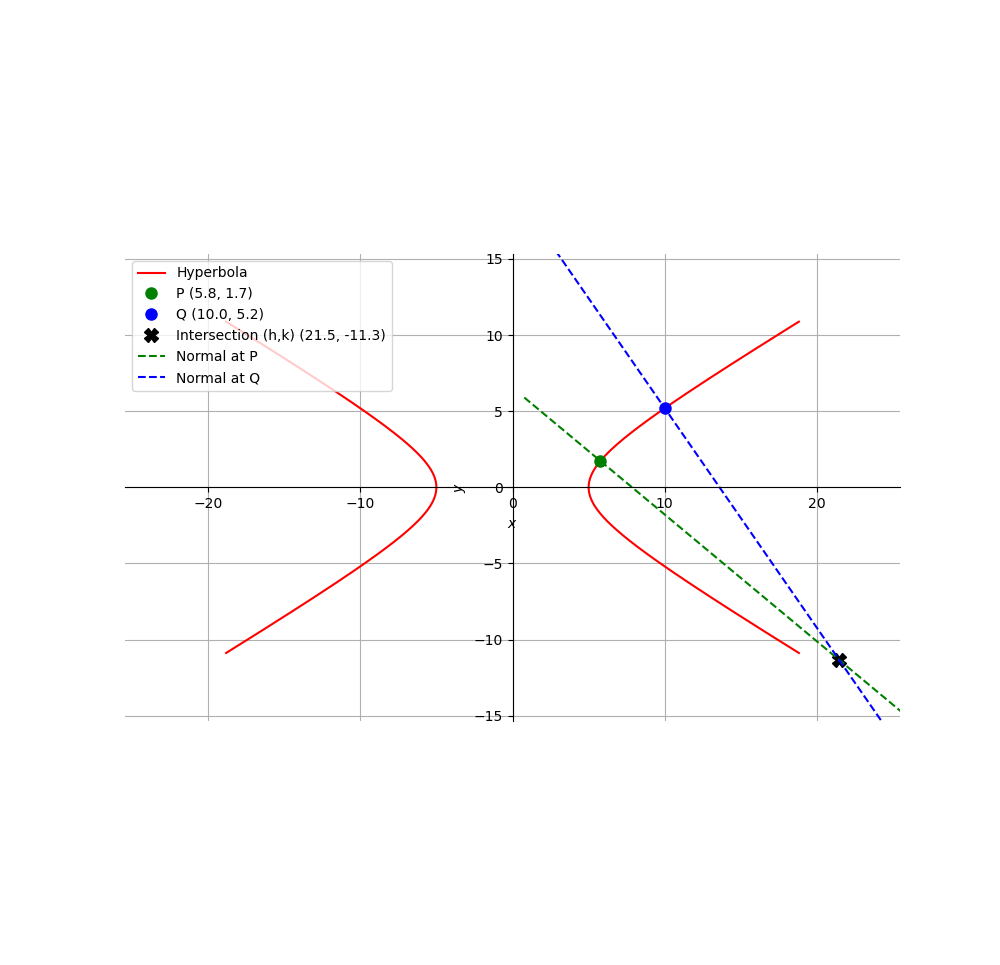
\includegraphics[width=0.7\columnwidth]{figs/Figure_1.png}
    \label{fig:placeholder}
    \caption{1}
\end{figure}
\end{frame}
\end{document}